\author{Tamlin Love - 1438243}
\title{Machine Learning Naive Bayes Tutorial}
\date{}
\documentclass[10pt]{article}

\usepackage{amsmath}
\usepackage{listings}
\usepackage{color}

\definecolor{dkgreen}{rgb}{0,0.6,0}
\definecolor{gray}{rgb}{0.5,0.5,0.5}
\definecolor{mauve}{rgb}{0.58,0,0.82}

\lstset{frame=tb,
  language=Python,
  aboveskip=3mm,
  belowskip=3mm,
  showstringspaces=false,
  columns=flexible,
  basicstyle={\small\ttfamily},
  numbers=none,
  numberstyle=\tiny\color{gray},
  keywordstyle=\color{blue},
  commentstyle=\color{dkgreen},
  stringstyle=\color{mauve},
  breaklines=true,
  breakatwhitespace=true,
  tabsize=3
}

\usepackage{graphicx}
\usepackage{float}
\graphicspath{ {.../Machine Learning/} }

\usepackage{amsmath}

\begin{document}
\maketitle
1.\\
a)\\
An list of short, 18 line reviews were passed in the following program, which used a random 12 of the reviews as training data and tested sentiment analysis on the other 6. The training reviews were broken up into words and these words were stored in an array, \textit{words}. Two other arrays, \textit{positiveCount} and \textit{negativeCount}, were used to the number of occurrences of each word in the positive and negative reviews respectively.\\
\\ 
Using Naive-Bayes (and Laplace smoothing where the occurrence of a word for a given sentiment was 0 or the word had not yet been encountered), the probability of a given sentiment (positive or negative) for a testing review's words was calculated.\\
\\
From this, a confusion matrix was created. The algorithm was run 1000 times and an average confusion matrix was created to better understand the performance of the algorithm.\\
\\
The code is shown below.
\begin{lstlisting}
import NBControl as nb
import numpy as np
from random import randint
from math import exp

reviewText = nb.readFile('simple-food-reviews.txt')
trainingNo = 12
bigConfusion = np.zeros([2,2])
bigIteration = 1000

for iteration in range(bigIteration):
    reviews = reviewText.split('\n')        #Split text into reviews

    #Generate a random list of 12 reviews for training
    trainingReviews = []
    for i in range(trainingNo):
        j = randint(0,len(reviews)-1)
        a = reviews.pop(j)
        trainingReviews.append(a)

    #Do training
    words = []
    positiveCount = []
    negativeCount = []
    positiveNo = 0
    negativeNo = 0
    totalNo = trainingNo

    for i in range(trainingNo):
        thisReviewWords = trainingReviews[i].split()        #Split review into its words
        thisSentiment = thisReviewWords[0]                  #Take sentiment
        if thisSentiment == "-1":
            negativeNo = negativeNo + 1
        else:
            positiveNo = positiveNo + 1
        for j in range(1,len(thisReviewWords)):
            if thisReviewWords[j] in words:
                index = words.index(thisReviewWords[j])
                if thisSentiment == "-1":
                    negativeCount[index] = negativeCount[index] + 1
                else:
                    positiveCount[index] = positiveCount[index] + 1
            else:
                words.append(thisReviewWords[j])
                if thisSentiment == "-1":
                    negativeCount.append(1)
                    positiveCount.append(0)
                else:
                    positiveCount.append(1)
                    negativeCount.append(0)


    #Do testing

    PNeg = 1.0*negativeNo/totalNo
    PPos = 1.0*positiveNo/totalNo
    totalCount = np.array(negativeCount)+np.array(positiveCount)
    k = 1
    nk = 2
    confusion = np.zeros([2, 2])
    for i in range(len(reviews)):
        thisReviewWords = reviews[i].split()    #Split review into words
        mySentiment = thisReviewWords.pop(0)
        runningProbPos = 1
        runningProbNeg = 1
        for j in range(len(thisReviewWords)):
            if thisReviewWords[j] not in words:
                runningProbNeg *= 1.0 * k / (negativeNo + nk)
                runningProbPos *= 1.0 * k / (positiveNo + nk)
        for j in range(len(words)):
            if words[j] in thisReviewWords:
                if negativeCount[j]==0:
                    runningProbNeg *= 1.0 * k / (negativeNo + nk)
                else:
                    runningProbNeg *= 1.0 * (negativeCount[j]) / (negativeNo)
                if positiveCount[j]==0:
                    runningProbPos *= 1.0 * k / (positiveNo + nk)
                else:
                    runningProbPos *= 1.0 * (positiveCount[j]) / (positiveNo)
            else:
                runningProbNeg *= 1.0 * (1 - (negativeCount[j] + k) / (negativeNo + nk))
                runningProbPos *= 1.0 * (1 - (positiveCount[j] + k) / (positiveNo + nk))
        print(runningProbNeg)
        negProb = 1.0 * (runningProbNeg * PNeg) / ((runningProbNeg * PNeg) + (runningProbPos * PPos))
        posProb = 1.0 * (runningProbPos * PPos) / ((runningProbNeg * PNeg) + (runningProbPos * PPos))
        if negProb >= posProb:
            prediction = '-1'
        else:
            prediction = '1'
        if prediction == mySentiment:
            if prediction == '1':
                confusion[0,0] += 1
            else:
                confusion[1,1] += 1
        else:
            if prediction == '1':
                confusion[0,1] += 1
            else:
                confusion[1,0] += 1
    bigConfusion += confusion

bigConfusion = np.divide(bigConfusion,bigIteration)
print(bigConfusion)
\end{lstlisting}
\newpage
After the code was run, the average confusion matrix produced looked like this:
\begin{table}[h]
\centering
\begin{tabular}{lll}
                   & Actually positive & Actually negative \\
Predicted positive & 1.814             & 1.631 \\
Predicted negative & 1.161             & 1.394            
\end{tabular}
\end{table}\\
This represents fairly poor accuracy of 53.47\%, which can be attributed to the tiny training data size and the over-emphasis on neutral words (such as \textit{the}, \textit{I} and \textit{we}, for example).\\
\\
b)\\
The code above was modified to use all 18 reviews for training, while additional reviews were inputted by the user. It was also modified to immediately output the prediction and probability of the sentiment given the review. A -1 would terminate the program. An example output is shown below:
\begin{figure}[H]
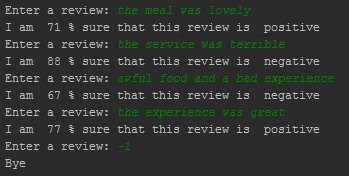
\includegraphics[scale=1]{RestaurantUserInputExample.png}
\end{figure}
\newpage
To confuse the program, the following inputs were given:
\begin{figure}[H]
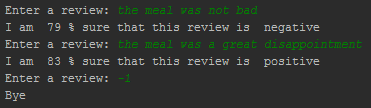
\includegraphics[scale=1]{RestaurantUserInputConfuseExample.png}
\end{figure}
In the first case, the word \textit{bad} indicated a negative review, which is false as the qualifier \textit{not} negates the word \textit{bad}. Not only did the word \textit{not} not appear in any of the training reviews, but the program was not equipped to deal with a change of meaning created by joining two words (\textit{not bad} is opposite to \textit{bad}).\\
\\
In the second case, the word \textit{great} indicated a positive review when in fact it merely described the word \textit{disappointment}, which indicates negativity. Once again, not only was \textit{disappointment} not in the training reviews, but the change of meaning when words are combined was not anticipated by the algorithm.\\
\\
c)\\
Modifying the code presented in Question 1 (a) to ignore all entries with 0 probability rather than applying Laplace-smoothing to them, the following average confusion matrix was generated:
\begin{table}[h]
\centering
\begin{tabular}{lll}
                   & Actually positive & Actually negative \\
Predicted positive & 0.763             & 1.597 \\
Predicted negative & 2.121             & 1.294            
\end{tabular}
\end{table}\\
This matrix indicates far worse performance (34.28\%) than the same algorithm with Laplace smoothing, demonstrating the positive effects of the technique.
\newpage
d)\\After modifying the program to ignore words of 2 characters or less, the following average confusion matrix was produced:
\begin{table}[h]
\begin{tabular}{lll}
                   & Actually positive & Actually negative \\
Predicted positive & 1.788             & 1.386 \\
Predicted negative & 1.206             & 1.62            
\end{tabular}
\end{table}\\
This matrix indicates moderately better performance (56.80\%) than the original one, suggesting that ignoring small words that are unlikely to contribute to the sentiment is a good idea.
\newpage
2.\\
The following code was used to perform sentiment analysis on a set of real movie reviews, with 90\% of the reviews used as training data and the remaining 10\% used as testing data. Laplace smoothing was employed, and words which appeared in testing reviews but not in training reviews were ignored.\\ 
\\
The use of a larger dataset was challenging as it forced the code to be optimized for performance. Dictionaries were used instead of simple lists as the time complexity for checking whether a value appears in a dictionary is \textit{O(1)}, as opposed to \textit{O(n)} for a list. Additionally, underflow became an issue when multiplying probabilities. To overcome this, the natural logarithm of each word's probability was taken and then added together. A high precision library, Decimal, was used to convert the logarithms back to the standard form for use in the Naive-Bayes formula.  
\begin{lstlisting}
import NBControl as nb
import numpy as np
from random import randint
from math import ceil
from math import log
from decimal import *

reviewText = nb.readFile('movie-pang02.csv')        #   Read reviews from file

#   Settings

trainingPercent = 0.9       #Percentage of reviews to be used for training
getcontext().prec = 100     #Precision of decimals

k = 1               #Laplace Smoothing Numerator
nk = 2              #Laplace Smoothing Denominator

bigConfusion = np.zeros([2, 2])
bigIter = 60

for iteration in range(bigIter):
    #   Generate list of reviews

    allReviews = reviewText.split('\n')     #Split text into reviews
    allReviews.pop(0)              #Remove table head
    trainingNo = int(ceil(trainingPercent*len(allReviews)))     #Exact number of reviews for training
    trainingReviews = []
    for i in range(trainingNo):
        j = randint(0, len(allReviews) - 1)
        a = allReviews.pop(j)
        trainingReviews.append(a)

    #   Training

    print 'Training begins on iteration ', iteration+1

    posNo = 0       #Number of positive reviews in training set
    negNo = 0       #Number of negative reviews in training set
    posWords = {}   #Dictionary of positive words
    negWords = {}   #Dictionary of negative words
    for i in range(trainingNo):
        #print 'Training Review #',i+1
        firstSplit = trainingReviews[i].split(',')          #Split the review into Sentiment and Text
        thisReviewWordsSet = set(firstSplit[1].split())     # Split review into a set of unique words
        thisReviewWords = list(thisReviewWordsSet)          # Create a list from the set
        mySentiment = firstSplit[0]                         #Take sentiment
        if mySentiment == 'Pos':
            posNo += 1
        else:
            negNo += 1
        for j in range(len(thisReviewWords)):
            negMod = 0
            posMod = 0
            if mySentiment == 'Pos':
                posMod = 1
            else:
                negMod = 1
            if thisReviewWords[j] in posWords:
                posWords[thisReviewWords[j]] += posMod
            else:
                posWords[thisReviewWords[j]] = posMod
            if thisReviewWords[j] in negWords:
                negWords[thisReviewWords[j]] += negMod
            else:
                negWords[thisReviewWords[j]] = negMod

    #   Testing
    print 'Testing begins on iteration ', iteration+1

    confusion = np.zeros([2, 2])
    posProb = 1.0*posNo/trainingNo
    negProb = 1.0*negNo/trainingNo

    for i in range(len(allReviews)):
        #print 'Testing Review #',i+1
        firstSplit = trainingReviews[i].split(',')          # Split the review into Sentiment and Text
        thisReviewWordsSet = set(firstSplit[1].split())     # Split review into a set of unique words
        thisReviewWords = list(thisReviewWordsSet)          #Create a list from the set
        mySentiment = firstSplit[0]                         # Take sentiment
        runningNeg = 0
        runningPos = 0
        wordCount = 0
        for j in posWords:
            if j in thisReviewWords:
                wordCount += 1
                runningPos += log(posWords[j]+k)-log(posNo+nk)
                runningNeg += log(negWords[j]+k)-log(negNo+nk)
            else:
                runningPos += log(1 - 1.0*(posWords[j]+k)/(posNo+nk))
                runningNeg += log(1 - 1.0*(negWords[j]+k)/(negNo+nk))

        #For this, we ignore words that are in review i but not in the dictionary, as the effect is minimal

        PNegPart = Decimal.exp(Decimal(runningNeg))*Decimal(negProb)
        PPosPart = Decimal.exp(Decimal(runningPos))*Decimal(posProb)
        PNeg = PNegPart/(PNegPart+PPosPart)
        PPos = PPosPart/(PNegPart+PPosPart)
        if PNeg >= PPos:
            prediction = 'Neg'
        else:
            prediction = 'Pos'
        if prediction == mySentiment:
            if prediction == 'Pos':
                confusion[0, 0] += 1
            else:
                confusion[1, 1] += 1
        else:
            if prediction == 'Pos':
                confusion[0, 1] += 1
            else:
                confusion[1, 0] += 1

    print 'Finished with iteration ', iteration+1
    bigConfusion += confusion
    intermediateConfusion = np.divide(bigConfusion, iteration+1)
    print 'Current confusion matrix: '
    print intermediateConfusion

bigConfusion = np.divide(bigConfusion, bigIter)
print 'Final confusion matrix: '
print bigConfusion
\end{lstlisting}
\newpage
The algorithm was repeated 60 times to produce an average confusion matrix, shown below.
\begin{table}[h]
\centering
\begin{tabular}{lll}
                   & Actually positive & Actually negative \\
Predicted positive & 91.23333333             & 0.4 \\
Predicted negative & 9.55             & 98.81666667            
\end{tabular}
\end{table}\\
This corresponds to 95.02\% accuracy, which is a very good result. It could potentially be improved by removing words of less than a certain length (for example, removing words of length less than three, as in question 1 (d) above).\\
\\
3.\\
The normal probability density function is given as
\begin{equation}
f(x_{i}|\mu,\sigma^2) = \frac{1}{\sqrt{2 \pi \sigma^{2}}}e^{-\frac{(x_{i}-\mu)^2}{2\sigma^2}}
\end{equation}
Now, given the assumption that each sampled observation is independent, we can express the likelihood function of the distribution as
\begin{equation}
\begin{array}{l@{{}={}}l}
L(\mu,\sigma^2 | \bar{x}) 
& \prod_{i=1}^{n} f(x_{i}|\mu,\sigma^2) \\
& \prod_{i=1}^{n} \frac{1}{\sqrt{2 \pi \sigma^{2}}}e^{-\frac{(x_{i}-\mu)^2}{2\sigma^2}} \\
& (2 \pi \sigma^{2})^{-\frac{n}{2}} e^{-\frac{1}{2\sigma^2}\sum_{i=1}^{n}(x_{i} - \mu)^2}
\end{array}
\end{equation}
We can simplify the likelihood function by taking its natural logarithm.
\begin{equation}
\begin{array}{l@{{}={}}l}
\ln(L(\mu,\sigma^2 | \bar{x})) 
& \ln((2 \pi \sigma^{2})^{-\frac{n}{2}} e^{-\frac{1}{2\sigma^2}\sum_{i=1}^{n}(x_{i} - \mu)^2}) \\
& \ln ((2 \pi \sigma^{2})^{-\frac{n}{2}}) + \ln(e^{-\frac{1}{2\sigma^2}\sum_{i=1}^{n}(x_{i} - \mu)^2}) \\
& -\frac{n}{2}[\ln(2\pi)+\ln(\sigma^2)] -\frac{1}{2\sigma^2}\sum_{i=1}^{n}(x_{i} - \mu)^2 
\end{array}
\end{equation}
Now, since we are looking for the maximum likelihood, we need to maximize the likelihood function, which is equivalent to maximizing Equation (3). In other words, we must set
\begin{equation}
\nabla \ln(L(\mu,\sigma^2 | \bar{x})) = 0
\end{equation}
Which of course is equivalent to setting
\begin{equation}
\frac{\partial}{\partial \mu} \ln(L(\mu,\sigma^2 | \bar{x})) = 0 
\end{equation}
and
\begin{equation}
\frac{\partial}{\partial \sigma^2} \ln(L(\mu,\sigma^2 | \bar{x})) = 0 
\end{equation}
\newpage
Solving first for Equation (5),
\begin{equation}
\begin{array}{l@{{}={}}l}
\frac{\partial}{\partial \mu} \ln(L(\mu,\sigma^2 | \bar{x}))
& \frac{\partial}{\partial \mu} (-\frac{n}{2}[\ln(2\pi)+\ln(\sigma^2)] -\frac{1}{2\sigma^2}\sum_{i=1}^{n}(x_{i} - \mu)^2) \\
& \frac{1}{\sigma^2}\sum_{i=1}^{n}(x_{i} - \mu)
\end{array}
\end{equation}
Since $\frac{1}{\sigma^2} \neq 0$, Equation (5) is only satisfied if
\begin{equation}
\sum_{i=1}^{n}(x_{i} - \mu) = 0
\end{equation}
Thus
\begin{equation}
\sum_{i=1}^{n}(x_{i}) - n\mu = 0
\end{equation}
And so, solving for $\mu$, we arrive at 
\begin{equation}
\mu = \frac{1}{n}\sum_{i=1}^{n}(x_{i})
\end{equation}
which is the sample mean.\\
\\
Similarly, we now solve Equation (6) for $\sigma^2$.
\begin{equation}
\begin{array}{l@{{}={}}l}
\frac{\partial}{\partial \sigma^2} \ln(L(\mu,\sigma^2 | \bar{x}))
& \frac{\partial}{\partial \sigma^2} (-\frac{n}{2}[\ln(2\pi)+\ln(\sigma^2)] -\frac{1}{2\sigma^2}\sum_{i=1}^{n}(x_{i} - \mu)^2) \\
&\frac{\partial}{\partial \sigma^2}(-\frac{n}{2}\ln(\sigma^2)) - \frac{\partial}{\partial \sigma^2}(\frac{1}{2\sigma^2}\sum_{i=1}^{n}(x_{i} - \mu)^2)\\
& -\frac{n}{2\sigma^2} -(\sum_{i=1}^{n}(x_{i} - \mu)^2))\frac{\partial}{\partial \sigma^2}\frac{1}{2\sigma^2}\\
&  -\frac{n}{2\sigma^2} + (\sum_{i=1}^{n}(x_{i} - \mu)^2))\frac{1}{2(\sigma^{2})^{2}}\\
& \frac{1}{2\sigma^2}(-n + \frac{1}{\sigma^2}\sum_{i=1}^{n}(x_{i} - \mu)^2))\\
& 0
\end{array}
\end{equation}
Again, $\frac{1}{\sigma^2} \neq 0$. Thus,
\begin{equation}
\frac{1}{\sigma^2}\sum_{i=1}^{n}(x_{i} - \mu)^2 - n = 0 
\end{equation}
And therefore
\begin{equation}
\sigma^2 = \frac{1}{n}\sum_{i=1}^{n}(x_{i} - \mu)^2
\end{equation}
which is the sample variance.
\newpage
4.\\
The following code was used to tell which digit was displayed on an 8 pixel by 8 pixel, binarized image of a digit, using Naive-Bayes with Laplace Smoothing.
\begin{lstlisting}
import NBControl as nb
import numpy as np
from random import randint
from math import ceil
from math import log
from decimal import *

digitText = nb.readFile('smalldigits.csv')        # Read digits from file

#   Settings

trainingPercent = 0.8       # Percentage of digits to be used for training
getcontext().prec = 100     # Precision of decimals

k = 1               # Laplace Smoothing Numerator
nk = 2              # Laplace Smoothing Denominator

bigConfusion = np.zeros([10, 10])
bigIter = 100

for iteration in range(bigIter):
    # Generate list of digits
    allDigits = digitText.split('\n')  # Split text into each digit
    trainingNo = int(ceil(trainingPercent * len(allDigits)))  # Exact number of digits for training
    trainingDigits = []
    for i in range(trainingNo):
        j = randint(0, len(allDigits) - 1)
        a = allDigits.pop(j)
        trainingDigits.append(a)

    # Training
    print 'Training begins on iteration #',iteration
    digitNo = np.zeros(10)          # List of number of occurrence of each digit
    pixelMaps = []                  # Create a list of arrays, each one of which will list occurences of pixels for a given digit
    for i in range(10):
        pixelMaps.append(np.zeros(64))

    for i in range(trainingNo):
        # print 'Training digit ',i+1
        thisDigit = trainingDigits[i].split(',')        # Split digit into individual pixels (64) + digit
        myDigit = int(thisDigit.pop(64))                # Get actual digit
        thisDigit = np.asarray(np.array(thisDigit),int)
        digitNo[myDigit] += 1
        pixelMaps[myDigit] += thisDigit                 # Add this digit's array to the count array

    # Testing
    print 'Testing begins on iteration #',iteration

    confusion = np.zeros([10,10])
    digitProbs = []
    for i in range(10):
        digitProbs.append(1.0*digitNo[i]/trainingNo)

    for i in range(len(allDigits)):
        # print 'Testing digit ',i+1
        thisDigit = trainingDigits[i].split(',')            # Split digit into individual pixels (64) + digit
        myDigit = int(thisDigit.pop(64))                    # Get actual digit
        runnings = np.zeros(10)
        for j in range(len(thisDigit)):
            if thisDigit[j] == '1':
                for m in range(10):
                    runnings[m] += log(pixelMaps[m][j]+k)-log(digitNo[m]+nk)
            else:
                for m in range(10):
                    runnings[m] += log(1 - 1.0*(pixelMaps[m][j]+k)/(digitNo[m]+nk))

        probPart = []
        denom = 0
        for j in range(10):
            number = Decimal.exp(Decimal(runnings[j]))*Decimal(digitProbs[j])
            probPart.append(number)
            denom += number

        myProb = []
        for j in range(10):
            myProb.append(probPart[j]/denom)

        prediction = myProb.index(max(myProb))
        confusion[prediction,myDigit] += 1

    print 'Finished with iteration ',iteration+1
    bigConfusion += confusion
    intermediateConfusion = np.divide(bigConfusion, iteration + 1)
    print 'Current confusion matrix: '
    print intermediateConfusion
    accuracy = 0
    for j in range(10):
        accuracy += intermediateConfusion[j, j]
    accuracy = 1.0 * accuracy / len(allDigits)
    print 'Current Accuracy = ', 100 * accuracy, '%'


bigConfusion = np.divide(bigConfusion, bigIter)
print 'Final confusion matrix: '
print bigConfusion
accuracy = 0
for j in range(10):
    accuracy += bigConfusion[j, j]
accuracy = 1.0*accuracy/len(allDigits)
print 'Accuracy = ', 100*accuracy, '%'
\end{lstlisting}
The algorithm was run 100 times to produce the following average confusion matrix.   
\begin{table}[h]
\centering
\begin{tabular}{lllllllllll}
            & 0     & 1     & 2     & 3     & 4     & 5     & 6     & 7     & 8     & 9     \\
Predicted 0 & 35.12 & 0.00  & 0.00  & 0.25  & 0.00  & 0.00  & 0.12  & 0.00  & 0.00  & 0.00  \\
Predicted 1 & 0.00  & 26.58 & 1.88  & 0.50  & 0.36  & 0.24  & 0.70  & 0.00  & 2.66  & 1.43  \\
Predicted 2 & 0.00  & 3.45  & 31.60 & 0.54  & 0.00  & 0.00  & 0.00  & 0.00  & 0.19  & 0.15  \\
Predicted 3 & 0.00  & 0.00  & 0.68  & 30.88 & 0.00  & 0.01  & 0.00  & 0.00  & 0.28  & 1.44  \\
Predicted 4 & 0.17  & 0.18  & 0.00  & 0.00  & 34.25 & 0.38  & 0.22  & 0.26  & 0.00  & 0.26  \\
Predicted 5 & 0.21  & 0.17  & 0.00  & 0.42  & 0.00  & 32.04 & 0.01  & 0.00  & 0.59  & 0.67  \\
Predicted 6 & 0.00  & 0.36  & 0.00  & 0.23  & 0.00  & 0.18  & 34.92 & 0.00  & 0.20  & 0.00  \\
Predicted 7 & 0.00  & 0.42  & 0.22  & 1.41  & 1.28  & 0.20  & 0.00  & 34.42 & 0.41  & 1.46  \\
Predicted 8 & 0.07  & 4.28  & 0.81  & 1.17  & 0.53  & 0.24  & 0.27  & 0.18  & 28.16 & 0.51  \\
Predicted 9 & 0.00  & 1.59  & 0.52  & 1.51  & 0.00  & 2.80  & 0.00  & 0.00  & 1.83  & 29.93
\end{tabular}
\end{table}\\
This corresponds to an accuracy of 88.55\%, which is very reasonable. A few common confusions include confusing 8 and 1, 2 and 1 and 9 and 3, all of which are likely due to the low resolution of the images. This may be improved by using a larger dataset and by using more detailed images (larger size and non-binarized). 
\end{document}